\documentclass[a4paper,14pt]{extarticle}

\usepackage[utf8x]{inputenc}
\usepackage[T1,T2A]{fontenc}
\usepackage[russian]{babel}
\usepackage{hyperref}
\usepackage{indentfirst}
\usepackage{here}
\usepackage{array}
\usepackage{graphicx}
\usepackage{caption}
\usepackage{subcaption}
\usepackage{chngcntr}
\usepackage{amsmath}
\usepackage{amssymb}
\usepackage{pgfplots}
\usepackage{pgfplotstable}
\usepackage[left=2cm,right=2cm,top=2cm,bottom=2cm,bindingoffset=0cm]{geometry}
\usepackage{multicol}

\renewcommand{\le}{\ensuremath{\leqslant}}
\renewcommand{\leq}{\ensuremath{\leqslant}}
\renewcommand{\ge}{\ensuremath{\geqslant}}
\renewcommand{\geq}{\ensuremath{\geqslant}}
\renewcommand{\epsilon}{\ensuremath{\varepsilon}}
\renewcommand{\phi}{\ensuremath{\varphi}}

\counterwithin{figure}{section}
\counterwithin{equation}{section}
\counterwithin{table}{section}
\newcommand{\sign}[1][5cm]{\makebox[#1]{\hrulefill}} % Поля подписи и даты
\graphicspath{{pics/}} % Путь до папки с картинками
\captionsetup{justification=centering,margin=1cm}
\def\arraystretch{1.3}

\begin{document}	% начало документа

\begin{titlepage}
\begin{center}
	\textbf{Санкт-Петербургский Политехнический Университет \\Петра Великого}\\[0.3cm]
	\small Институт компьютерных наук и технологий \\[0.3cm]
	\small Кафедра компьютерных систем и программных технологий\\[4cm]
	
	\textbf{ОТЧЕТ}\\ \textbf{о лабораторной работе}\\[0.5cm]
	\textbf{<<Исследование частотных характеристик пассивных RC-цепей>>}\\[0.1cm]
	\textbf{Электротехника и Электроника}\\[10.5cm]
\end{center}

\begin{flushright}
	\begin{minipage}{0.60\textwidth}
		\begin{flushleft}
			\small \textbf{Работу выполнили студенты}\\[3mm]
			\small группа 23501/4 \hspace*{17mm} Дьячков В.В.\\[3mm]
			\small группа 23501/4 \hspace*{17mm} Ламтев А.Ю.\\[5mm]
			
			\small \textbf{Преподаватель}\\[5mm]
		 	\small \sign[3.5cm] \hspace*{8mm} к.т.н., доц. Кочетков Ю.Д.\\[0.5cm]
		\end{flushleft}
	\end{minipage}
\end{flushright}

\vfill

\begin{center}
	\small Санкт-Петербург\\
	\small \the\year
\end{center}
\end{titlepage}


\section{Цель работы}

Рассчитать и исследовать экспериментально различных схем выпрямителей на полупроводниковых диодах и сглаживающих фильтрах.

\section{Чертеж схемы исследуемого устройства}

\begin{figure}[h]
\centering
\begin{subfigure}[b]{0.35\textwidth}
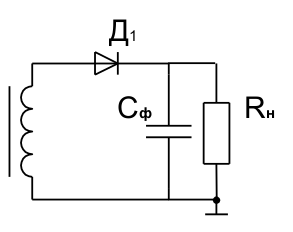
\includegraphics[scale=0.85]{diod.png}
\caption{Однополупериодный \\выпрямитель}\label{figure:2.1:a}
\end{subfigure}
\begin{subfigure}[b]{0.35\textwidth}
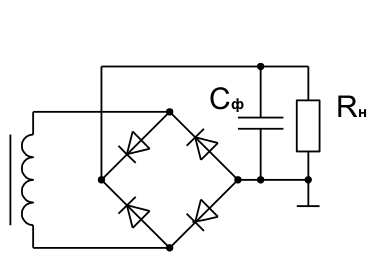
\includegraphics[scale=0.5]{4diods.png}
\caption{Двухполупериодный \\мостовой выпрямитель}\label{figure:2.1:b}
\end{subfigure}
\end{figure}

\section{Исходные данные}

$I_\text{н} = 120$ мА

$R_\text{изм} = 15$ Ом

$R_\text{н} = 470$ Ом

$C_\text{ф} = 1500$ мкФ

\section{Теоретические зависимости}



\section{Экспериментально снятые зависимости}

\subsection{Полупроводниковый диод}

\begin{table}[H]
	\begin{center}
	\caption{ВАХ полупроводникового диода}
	\def\arraystretch{1.2}
		\begin{tabular}{|c|c|c|c|c|}
		\hline 
		$U_1$, В & $U_2$, В & $U_\text{диода} = U_1 - U_2$, В & $U_\text{изм}$, В & $I_\text{диода}$, мА \\ 
		\hline 
		5.23 & 4.75 & 0.48 & 0.14 & 9.3 \\ 
		\hline 
		5.21 & 4.68 & 0.53 & 0.44 & 29.3 \\ 
		\hline 
		5.20 & 4.63 & 0.57 & 0.73 & 49.3 \\ 
		\hline 
		5.19 & 4.59 & 0.60 & 1.04 & 69.3 \\ 
		\hline 
		5.18 & 4.56 & 0.62 & 1.35 & 89.3 \\ 
		\hline 
		5.17 & 4.53 & 0.70 & 1.61 & 109.3 \\ 
		\hline 
		5.16 & 4.51 & 0.65 & 1.97 & 129.3 \\ 
		\hline 
		5.15 & 4.49 & 0.66 & 2.24 & 149.3 \\ 
		\hline 
		5.14 & 4.46 & 0.68 & 2.58 & 169.3 \\ 
		\hline 
		5.14 & 4.44 & 0.7 & 2.81 & 189.3 \\ 
		\hline 
		5.12 & 4.41 & 0.68 & 2.98 & 209.3 \\ 
		\hline 
		5.11 & 4.40 & 0.71 & 3.19 & 229.3 \\ 
		\hline 
		5.10 & 4.38 & 0.72 & 3.52 & 249.3 \\ 
		\hline 
		5.10 & 4.37 & 0.73 & 3.91 & 269.3 \\ 
		\hline 
		5.09 & 4.33 & 0.76 & 4.64 & 289.3 \\ 
		\hline 
		\end{tabular} 
		\label{tab:5:1}
	\end{center}
\end{table}

\subsection{Однополупроводникового выпрямитель}

\begin{table}[H]
	\begin{center}
	\caption{ВАХ однополупроводникового выпрямителя}
	\def\arraystretch{1.2}
		\begin{tabular}{|c|c|c|c|}
		\hline 
		$U_\text{изм}$, В & $I_\text{н}$, А & $U_\text{п}$, В & $U_\text{н}$, В \\ 
		
		\hline 
		0.25 & 0.02	& 9.28 & 0.20 \\ 
		\hline 
		0.60 & 0.04	& 9.08 & 0.43 \\ 
		\hline 
		0.90 & 0.06	& 9.01 & 0.61 \\ 
		\hline 
		1.20 & 0.08	& 8.84 & 0.77 \\ 
		\hline 
		1.51 & 0.10	& 8.79 & 0.98 \\ 
		\hline 
		1.83 & 0.12	& 8.50 & 1.13 \\ 
		\hline 
		2.15 & 0.14	& 8.40 & 1.29 \\ 
		\hline 
		2.41 & 0.16	& 8.24 & 1.56 \\ 
		\hline 
		2.70 & 0.18	& 8.15 & 1.62 \\ 
		\hline 
		3.03 & 0.20	& 8.09 & 1.80 \\ 
		\hline 
		3.25 & 0.22	& 7.99 & 1.92 \\ 
		\hline 
		3.68 & 0.25	& 7.81 & 2.12 \\ 
		\hline 
		4.00 & 0.27	& 7.70 & 2.28 \\ 
		\hline 
		4.35 & 0.29	& 7.49 & 2.48 \\ 
		\hline 
		6.61 & 0.44	& 6.97 & 3.60 \\ 
		\hline 
		6.79 & 0.45 & 6.93 & 3.64 \\ 
		\hline 
		\end{tabular} 
		\label{tab:5:1}
	\end{center}
\end{table}

\section{Погрешности}

  
\section{Выводы}


\end{document}
